% Created 2011-08-22 Mon 11:27
\documentclass[11pt]{article}
%\usepackage[utf8]{inputenc}
\usepackage[T1]{fontenc}
\usepackage{graphicx}
\usepackage{longtable}
\usepackage{hyperref}
\usepackage{comment}
\usepackage{booktabs}
\usepackage{color}
\usepackage{pgf}
\usepackage{tikz}
\usetikzlibrary{arrows,positioning,fit,shapes,decorations,decorations.pathmorphing,decorations.pathreplacing,calc,patterns,scopes,matrix}
\pgfrealjobname{patchapi}

\usepackage{helvet}
\usepackage{enumitem}
\usepackage[letterpaper]{geometry}
\usepackage{listings}
\usepackage{verbatim}
\usepackage[T1]{fontenc}

\setlength{\parindent}{0.0in}
\setlength{\parskip}{0.1in}

\newenvironment{apient}{\small\verbatim}{\endverbatim}

\newcommand{\apidesc}[1]{%
{\addtolength{\leftskip}{4em}%
#1\par\medskip}
}

\begin{document}
\thispagestyle{empty}

\begin{titlepage}
\beginpgfgraphicnamed{titlepage}
\begin{tikzpicture}[remember picture, overlay]
    \path
        (current page.north west) coordinate (origin)
        (current page.north) coordinate (topcenter);

    % Header
    \node [font=\sffamily] (pppt) at ($(topcenter) - (0,1.0in)$) 
        {\fontsize{24}{36}\selectfont Paradyn Parallel Performance Tools};

    % Document Title
% older versions of pgf have a bug for matrices in overlay mode;
% have to specify positions manually
%    \matrix (Title) [%
%        matrix of nodes,%
%        nodes={font=\sffamily,right},%
%        matrix anchor=west,%
%        row sep=12pt
%        ] at ($(origin)+(0.75in,-3.0in)$)
%    {
%        \fontsize{48}{56}\selectfont ParseAPI \\
%        \fontsize{44}{56}\selectfont Programmer's Guide \\
%    };

    \node [anchor=west,font=\sffamily] (title1) at ($(origin)+(0.75in,-3.0in)$)
        {\fontsize{48}{56}\selectfont PatchAPI};
    \node [anchor=west,font=\sffamily] (title2) at ($(title1.west)+(0in,-56pt)$)
        {\fontsize{48}{56}\selectfont Programmer's Guide};

    % Release information
%    \matrix (Releaseinfo) [%
%        matrix of nodes,%
%        nodes={font=\sffamily,right},%
%        matrix anchor=west,%
%        row sep=8pt
%        ] at ($(origin)+(0.75in,-5.0in)$)
%    {
%        %\fontsize{24}{32}\selectfont Release 0.1 \\
%        \fontsize{24}{32}\selectfont Beta Release \\
%        \fontsize{24}{32}\selectfont Oct 2010 \\
%    };

    \node [anchor=west,font=\sffamily] (rel1) at ($(origin)+(0.75in,-5.0in)$)
        {\fontsize{24}{32}\selectfont 1.0b Release};
    \node [anchor=west,font=\sffamily] (rel2) at ($(rel1.west)+(0in,-32pt)$)
        {\fontsize{24}{32}\selectfont Aug 2011};

    % Contact information
%    \matrix (UWaddress) [%
%        matrix of nodes,%
%        nodes={font=\sffamily\large,right},%
%        matrix anchor=north west
%        ] at ($(origin)+(0.75in,-7in)$)
%    {
%        Computer Science Department \\
%        University of Wisconsin--Madison \\
%        Madison, WI 53711 \\
%    };

    \node [anchor=west,font=\sffamily\large] (uw1) at ($(origin)+(0.75in,-7.0in)$)
        {Computer Science Department};
    \node [anchor=west,font=\sffamily\large] (uw2) at ($(uw1.west)+(0in,-20pt)$)
        {University of Wisconsin--Madison};
    \node [anchor=west,font=\sffamily\large] (uw3) at ($(uw2.west)+(0in,-20pt)$)
        {Madison, WI 53711};


%    \matrix (UMDaddress) [%
%        matrix of nodes,%
%        nodes={font=\sffamily\large,right},%
%        matrix anchor=north west,
%        below=1em of UWaddress.south west
%        ]
%    {
%        Computer Science Department \\
%        University of Maryland \\
%        College Park, MD 20742 \\
%    };

    \node [anchor=west,font=\sffamily\large] (umd1) at ($(uw3.south west)+(0in,-2.5em)$)
        {Computer Science Department};
    \node [anchor=west,font=\sffamily\large] (umd2) at ($(umd1.west)+(0in,-20pt)$)
        {University of Maryland};
    \node [anchor=west,font=\sffamily\large] (umd3) at ($(umd2.west)+(0in,-20pt)$)
        {College Park, MD 20742};

%    \matrix (Emails) [%
%        matrix of nodes,%
%        nodes={font=\sffamily,right},%
%        matrix anchor=north west,%
%        below=1em of UMDaddress.south west,%
%        anchor=base
%        ]
%    {
%        Email & \texttt{bugs@dyninst.org} \\
%        Web & \texttt{www.dyninst.org} \\
%    };

    \node [anchor=west,font=\sffamily] (email1) at ($(umd3.south west)+(-0.5em,-2.5em)$)
        %{Email \texttt{bugs@dyninst.org}};
        {\begin{tabular}{ll}%
         Email & \texttt{bugs@dyninst.org} \\
         Web & \texttt{www.dyinst.org} \\
        \end{tabular}};
        

    % Logo
    \path 
        node (logo) at ($(origin)+(4.0in,-7.0in)$) [%
            anchor=north west]
        {%
            
\includegraphics[width=3.25in]{paradyn_logo}
        }; 


\end{tikzpicture}
\endpgfgraphicnamed
\end{titlepage}

\tableofcontents
\clearpage

\section{Introduction}
\label{sec-1}

This manual describes PatchAPI, a programming interface and library
for binary code patching. A programmer uses PatchAPI to instrument
(insert code into) and modify a binary executable or library by
manipulating the binary's control flow graph (CFG). We allow the user
to instrument a binary by annotating a CFG with \emph{snippets}, or
sequences of inserted code, and to modify the binary by directly
manipulating the CFG. The PatchAPI interface, and thus tools written
with PatchAPI, is designed to be flexible and extensible. First, users
may \emph{inherit} from PatchAPI abstractions in order to store their
own data. Second, users may create \emph{plugins} to extend PatchAPI
to handle new types of instrumentation, different binary types, or
different patching techniques. 

PatchAPI represents the binary as an annotatable and modifiable
CFG. The CFG consists of four primary abstractions, which are similar
to the CFG abstractions used by the ParseAPI component:
\begin{description}
\item[PatchBlock:] A PatchBlock represents a single basic block, a
  contiguous sequence of instructions that are executed as a single
  unit. These objects form the nodes of our CFG. 
\item[PatchEdge:] A PatchEdge represents a possible control flow path
  between two PatchBlocks. PatchEdges are \emph{typed} to represent
  when the edge is traversed. 
\item[PatchFunction:] A PatchFunction represents a collection of
  PatchBlocks that are analogous to a source function. There is not
  always a clear mapping between source functions and functions in the
  binary due to compiler optimizations (e.g., function inlining). We
  define a function as the collection of blocks between a unique
  \emph{entry block} and an \emph{exit block} that contains a return
  instruction. As a result, functions may \emph{overlap} and contain
  a common subset of blocks; an example of this can be found in the
  ParseAPI documentation.
\item[PatchObject:] A PatchObject represents a binary file (or its
  memory equivalent), and represents a ParseAPI CodeObject.
\end{description}

Users instrument the binary by annotating this CFG using three
additional abstractions:
\begin{description}
\item[Point]: A Point supports instrumentation by representing a
  particular aspect of program behavior (e.g., entering a function or
  traversing an edge) and containing instances of Snippets. We define
  several classes of Points, as can be seen in Figure \ref{Points}.
\item[Snippet]: A Snippet represents a sequence of inserted code. To
  maximize flexibility, PatchAPI does not prescribe a particular
  snippet form; instead, users may provide their own (e.g., a binary
  buffer, a Dyninst abstract syntax tree (AST), or code written in the
  DynC language). Users instrument the binary by adding Snippets to
  the desired Points. 
\item[Instance]: An Instance represents the insertion of a particular
  Snippet at a particular Point.
\end{description}

Point lookup is performed with a single PatchAPI manager (PatchMgr)
object. This object represents a binary along with all of its
dependent libraries. Points are looked up in the manager by Scope
(e.g., a CFG object) and Type (e.g., function entry). In addition, a
user may provide an optional Filter which selects a subset of matching
Points.

The following C++ code snippet demonstrates the Point/Snippet
interface:

\begin{verbatim}
// We are interested in instrumenting a function, block, and edge
PatchFunction *func = ...;
PatchBlock *block = ...;
PatchEdge *edge = ...;

// Point lookup is done via a manager (PatchMgr) object
PatchMgr *mgr = ...;

// Find the following points: function entry, function exit,
// pre-call (immediately before a call is executed), block entry,
// and edge traversal

PointVector pts;

mgr->findPoints(Scope(func),
                Point::FuncEntry | 
                Point::PreCall | 
                Point::FuncExit,
                back_inserter(pts));
mgr->findPoints(Scope(block),
                Point::BlockEntry,
                back_inserter(pts));
mgr->findPoints(Scope(edge),
                Point::EdgeDuring,
                back_inserter(pts));

// Insert a single Snippet at each Point
Snippet::ptr snippet = ...;

for (PointVector::iterator iter = pts.begin(); 
     iter != pts.end(); ++iter) {
  (*iter)->push_back(snippet);
}

// For efficiency, we can batch instrumentation
mgr->commit();

\end{verbatim}


The core PatchAPI representation of an annotatable and modifiable CFG
operates in several domains, including on a running process (dynamic
instrumentation) or a file on disk (binary rewriting). Furthermore,
PatchAPI may be used both in the same address space as the process
(1st-party instrumentation) or in a different address space via the
debug interface (3rd-party instrumentation). Similarly, developers may
define their own types of Snippets to encapsulate their own code
generation techniques. These capabilities are provided by a plugin
interface; by implementing a plugin a developer may extend PatchAPI's
capabilities. The core plugin abstractions are:

\begin{description}
\item[AddressSpace]: An AddressSpace defines the low-level mechanisms
  necessary to manipulate a process or binary, including reading,
  writing, and allocating new memory.
\item[Snippet Generator]: A Snippet Generator defines how to convert a
  provided Snippet into the binary code that is injected into the
  process.
\item[Code Parser]: The Code Parser is responsible for creating the
  PatchAPI CFG. 
\item[Instrumentation Engine]: An Instrumentation Engine is
  responsible for generating the instrumented binary, including all
  CFG modifications and inserted snippets.
\end{description}



\section{Abstractions}
\label{sec-2}

\begin{figure}[htb]
\centerline{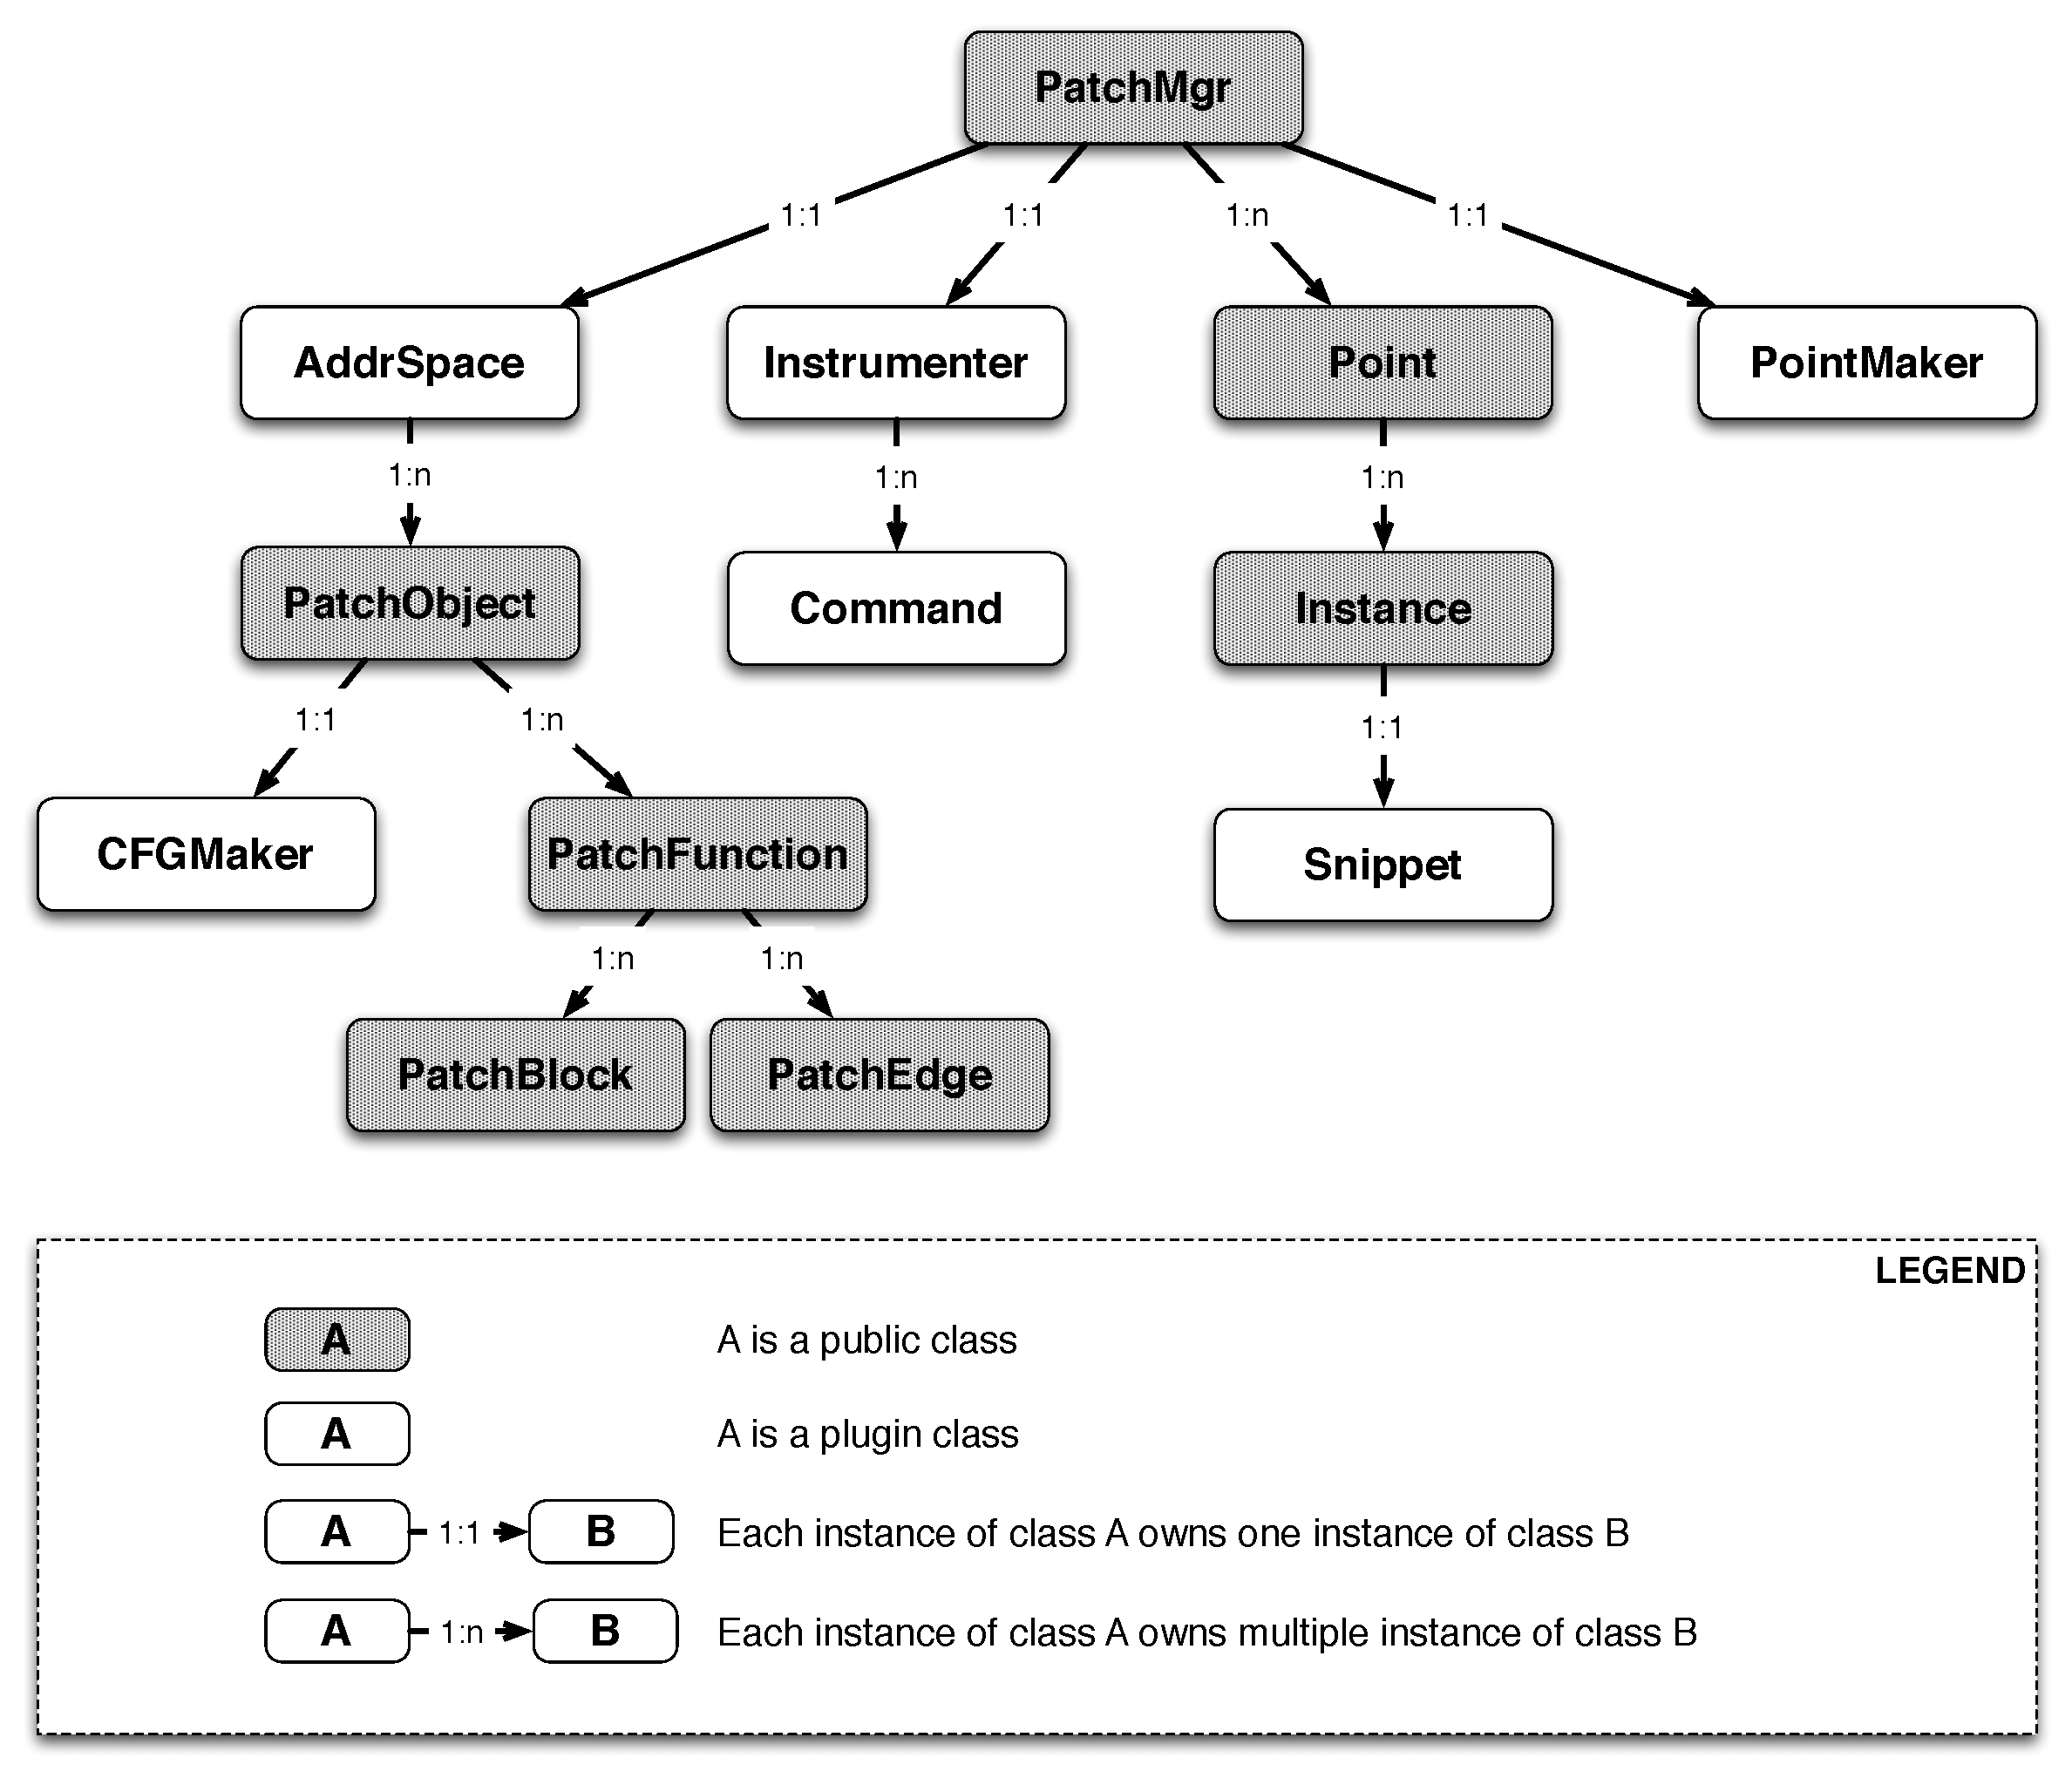
\includegraphics[width=0.85\textwidth]{./figure/abstraction/img.pdf}}
\caption{\label{fig:abs}Object Ownership}
\end{figure}


PatchAPI contains two interfaces: the public interface and the plugin interface.
The public interface is used to find instrumentation points, insert / delete
code snippets, and register plugins provided by programmers. The plugin
interface is used to customize different aspects in the binary code patching.
PatchAPI provides a set of default plugins for first party code patching, which
is easy to extend to meet different requirements in practice.

Figure \ref{fig:abs} shows the ownership hierarchy for PatchAPI's classes.
Ownership is a ``contains'' relationship. If one class owns another, then
instances of the owner class maintain exactly one or possibly more than one
instances of the other, which depends whether the relationship is a ``1:1'' or a
``1:n'' relationship. In Figure \ref{fig:abs}, for example, each PatchMgr instance
contains exactly one instance of a AddrSpace object, while a PatchMgr may
contains more than one instances of a Point object.

The remainder of this section briefly describes the classes that make up
PatchAPI's two interfaces. For more details, see the class descriptions in the
next section.
\subsection{Public Interface}
\label{sec-2.1}

PatchMgr, Point, and Snippet are used to perform the main process of binary code
patching: 1) find some \textbf{Point}; 2) insert or delete \textbf{Snippet} at some \textbf{Point}.
\begin{itemize}
\item \emph{PatchMgr} - The PatchMgr class is the top-level class for finding
    instrumentation \textbf{Points}, inserting or deleting \textbf{Snippets}, and registering
    user-provided plugins.
\item \emph{Point} - The Point class represents a location on the CFG that acts as a
    container of inserted snippet \textbf{Instances}. Points of different types are
    distinct even the underlying code relocation and generation engine happens
    to put instrumentation from them at the same place.
\item \emph{Instance} - The Instance class is a representation of a particular snippet
    inserted at a particular point.
\end{itemize}
\subsection{Plugin Interface}
\label{sec-2.2}

The address space abstraction determines whether the code patching is 1st party,
3rd party or binary rewriting.
\begin{itemize}
\item \emph{AddrSpace} - The AddrSpace class represents the address space of a
    \textbf{Mutatee}, where it contains a collection of \textbf{PatchObjects} that represent
    shared libraries or a binary executable. In addition, programmers implement
    some memory management interfaces in the AddrSpace class to determines the
    type of the code patching - 1st party, 3rd party, or binary rewriting.
\end{itemize}
Programmers can decide the representation of a \textbf{Snippet}, for example, the
representation can be in high level language (e.g., C or C++), or can simply be
in binary code (e.g., 0s and 1s).
\begin{itemize}
\item \emph{Snippet} - The Snippet class is a template class, so that programmers can
    easily plug in their own snippet representation and the corresponding
    mini-compiler to translate the representation into the binary code.
\end{itemize}
PatchAPI provides a thin layer on top of ParseAPI's Control Flow Graph (CFG)
layer, which associates some usefully information for the ease of binary code
patching, for example, a shared library's load address. This layer of CFG
structures include PatchObject, PatchFunction, PatchBlock and PatchEdge classes.
Programmers can extend these four CFG classes, and use the derived class of
CFGMaker to build a CFG, so that programmers have the freedom to decide when to
parse the binary code into CFG structures.
\begin{itemize}
\item \emph{PatchObject} - The PatchObject class is a wrapper of ParseAPI's CodeObject
    class, which represents an individual binary code object, such as an
    executable or a library.
\item \emph{PatchFunction} - The PatchFunction class is a wrapper of ParseAPI's
    Function class, which represents a function.
\item \emph{PatchBlock} - The PatchBlock class is a wrapper of ParseAPI's Block class,
    which represents a basic block.
\item \emph{PatchEdge} - The PatchEdge class is a wrapper of ParseAPI's Edge class,
    which join two basic blocks in the CFG, indicating the type of control flow
    transfer instruction that joins the basic blocks to each other.
\item \emph{CFGMaker} - The CFGMaker class is a factory class that constructs the above
    CFG structures. Programmers can use this class to decide when to parse the
    binary code into CFG structures, e.g., to parse during the runtime of code
    patching or to reuse the previously parsed result.
\end{itemize}
\begin{figure}[htb]
\centerline{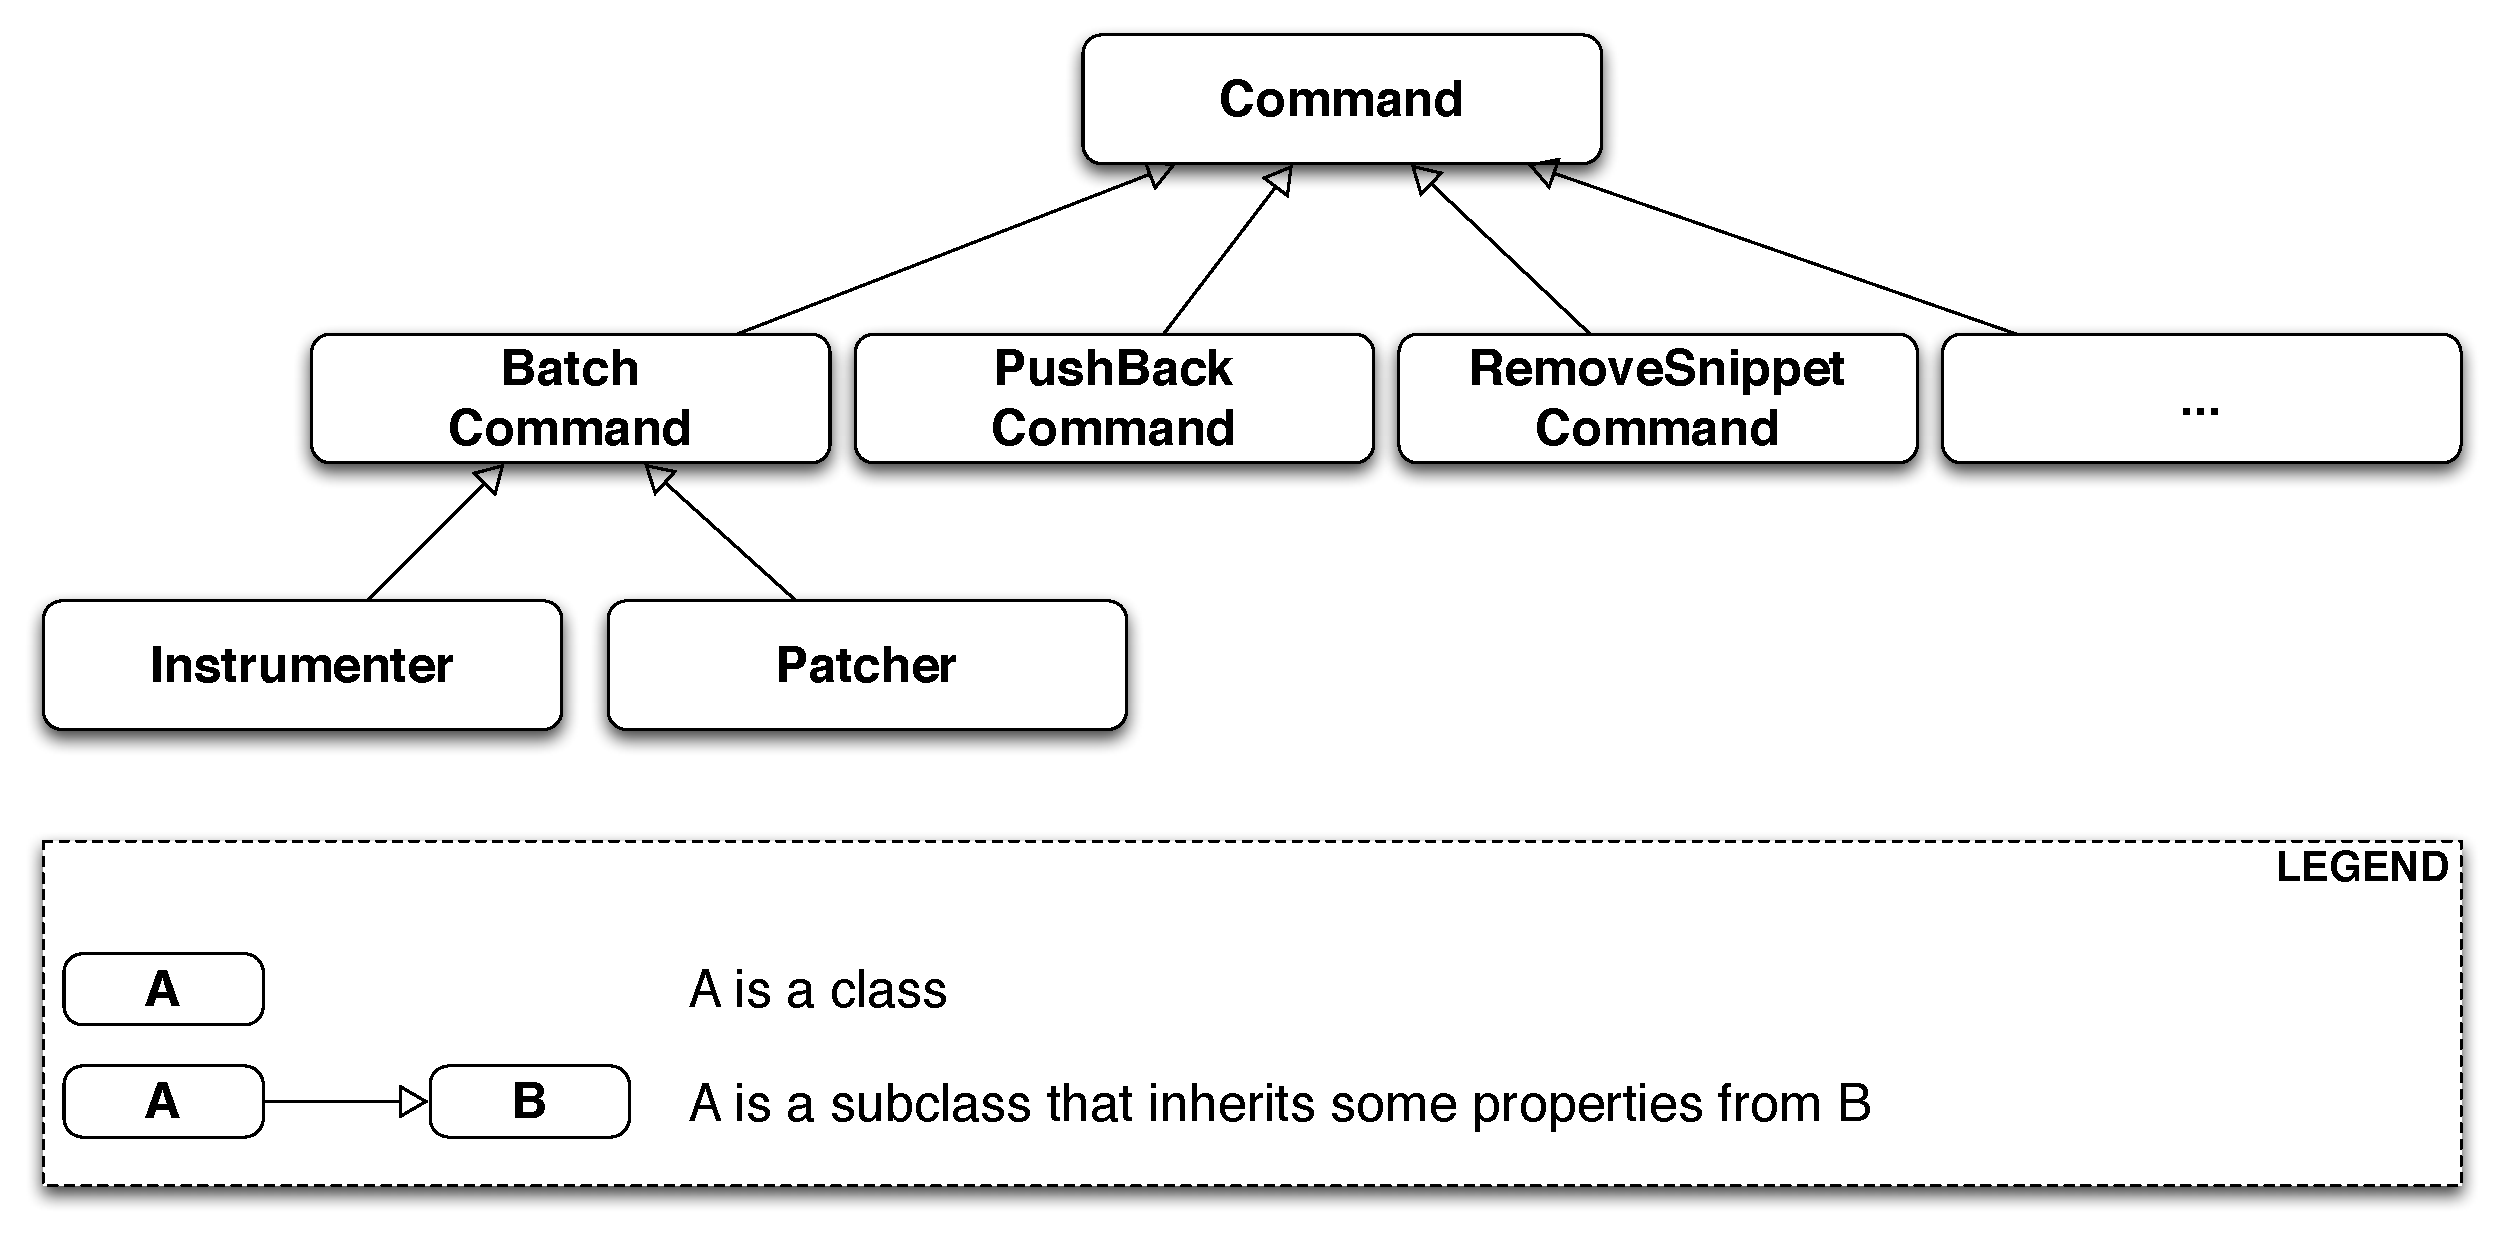
\includegraphics[width=0.85\textwidth]{./figure/command/img.pdf}}
\caption{\label{fig:inh}Inheritance Hierarchy}
\end{figure}


The implementation of an instrumentation engine may be very sophisticated (e.g.,
relocating a function), or be very simple (e.g., simply overwrite an
instruction). Therefore, PatchAPI provides a flexible framework for programmers
to customize the instrumentation engine. This framework is based on Command
Pattern. The instrumentation engine has transactional semantics, where all
instrumentation requests should succeed or all should fail. In our framework,
the \textbf{Command} abstraction represents an instrumentation request or a logical
step in the code patching process. We accumulate a list of \textbf{Commands}, and
execute them one by one. If one \textbf{Command} fails, we undo all executed
\textbf{Commands}. Figure \ref{fig:inh} illustrates the inheritance hierarchy for
related classes. There is a default implementation of instrumentation engine in
PatchAPI for 1st party code patching.
\begin{itemize}
\item \emph{Command} - The Command class represents an instrumentation request (e.g.,
    snippet insertion or removal), or a logical step in the code patching (e.g.,
    install instrumentation). This class provides a run() method and an undo()
    method, where run() will be called for normal execution, and undo() will be
    called for undoing this Command.
\item \emph{BatchCommand} - The BatchCommand class is a subclass of Command, and it is
    in fact a container of a list of Commands to be executed atomically.
\item \emph{Instrumenter} - The Instrumenter class inherits BatchCommand to encapsulate
    the core code patching logic, which includes binary code generation.
    Instrumenter would contain several logical steps that are individual
    Commands.
\item \emph{Patcher} - The Patcher class is also a subclass of BatchCommand. It accepts
    instrumentation requests from users, where these instrumentation requests
    are Commands (e.g., snippet insertion). Furthermore, Patcher implicitly adds
    Instrumenter to the end of the Command list to generate binary code and
    install the instrumentation.
\end{itemize}
\section{API Reference}
\label{sec-3}

This section describes functions in PatchAPI. The API is organized as a
collection of C++ classes. The classes in PatchAPI fall under the C++ namespace
Dyninst::PatchAPI. To access them, programmers should refer to them using the
``Dyninst::PatchAPI::'' prefix, e.g., Dyninst::PatchAPI::Point. Alternatively,
programmers can add the C++ \emph{using} keyword above any references to PatchAPI
objects, e.g.,/using namespace Dyninst::PatchAPI/ or \emph{using Dyninst::PatchAPI::Point}.

Most classes in PatchAPI use boost shared pointer (\emph{boost::shared$_{\mathrm{ptr}}$<T>}) for
memory management, where we typedef a class's shared pointer by appending the
Ptr to the class name, e.g., PatchMgrPtr for PatchMgr.

\subsection{Public Interface}
\label{sec-3.1}

\subsubsection{PatchMgr}
\label{sec-3.1.1}

\textbf{Declared in}: PatchMgr.h

The PatchMgr class is the top-level class for finding instrumentation \textbf{Points},
inserting or deleting \textbf{Snippets}, and registering user-provided plugins.


\begin{verbatim}
static PatchMgrPtr create(AddrSpacePtr as,
                          PointMakerPtr pf = PointMakerPtr(new PointMaker),
                          InstrumenterPtr inst = InstrumenterPtr());

\end{verbatim}



This factory method creates a new PatchMgr object that performs binary code
patching. It takes input three plugins, including AddrSpace \emph{as}, PointMaker
\emph{pf}, and Instrumenter \emph{inst}. PatchAPI uses default plugins for PointMaker and
Instrumenter, if \emph{pf} and \emph{inst} are not specified.

This method returns PatchMgrPtr() if it was unable to create a new PatchMgr
object.


\begin{verbatim}
struct Location {
  Location(PatchFunction *f, PatchBlock *b);
  Location(PatchFunction *f, InsnLoc l);
  Location(PatchFunction *f, PatchBlock *b, Address a,
           InstructionAPI::Instruction::Ptr i);
  Location(PatchFunction *f, PatchEdge *e);
  Location(PatchBlock *b);
  Location(InsnLoc l);
  Location(PatchBlock *b, Address a);
  Location(PatchEdge *e);

  typedef enum {
    Function,
    Block,
    BlockInstance,
    Instruction,
    InstructionInstance,
    Edge,
    Entry,
    Call,
    Exit,
    Illegal
  } type_t;

  bool legal(type_t t);

  PatchFunction *func;
  PatchBlock *block;
  Address addr;
  InstructionAPI::Instruction::Ptr insn;
  PatchEdge *edge;
  bool untrusted;
  type_t type;
};

\end{verbatim}



The Location structure uniquely identifies the physical location of a point.  A
Location object plus a Point::Type value uniquely identifies a point, because
multiple Points with different types can exist at the same physical location.


\begin{verbatim}
enum Point::Type {
  PreInsn,
  PostInsn,
  BlockEntry,
  BlockExit,
  BlockDuring,
  FuncEntry,
  FuncExit,
  FuncDuring,
  EdgeDuring,
  PreCall,
  PostCall,
  OtherPoint,
  None,
  InsnTypes = PreInsn | PostInsn,
  BlockTypes = BlockEntry | BlockExit | BlockDuring,
  FuncTypes = FuncEntry | FuncExit | FuncDuring,
  EdgeTypes = EdgeDuring,
  CallTypes = PreCall | PostCall
};

\end{verbatim}



The enum Point::Type specifies the logical point type.


\begin{verbatim}
Point *findPoint(Location loc,
                 Point::Type type,
                 bool create = true);

\end{verbatim}



This method returns a unique Point according to a Location \emph{loc} and a Type
\emph{type}. If we cannot find a Point, this method returns NULL. PatchAPI creates
Points on demand, so if a Point is not yet created, and the \emph{create} parameter
is false, this method returns NULL.


\begin{verbatim}
template <class OutputIterator>
bool findPoint(Location loc,
               Point::Type type,
               OutputIterator outputIter,
               bool create = true);

\end{verbatim}



This method finds a Point at a physical Location \emph{loc} with a \emph{type}.  It adds
the found Point to \emph{outputIter} that is a STL inserter.

This method returns true if a point is found, or the \emph{create} parameter is
false; otherwise, it returns false.


\begin{verbatim}
template <class OutputIterator>
bool findPoints(Location loc,
                Point::Type types,
                OutputIterator outputIter,
                bool create = true);

\end{verbatim}



This method finds Points at a physical Location \emph{loc} with composite \emph{types}
that are combined using the overloaded operator ``|''. This function outputs
Points to the STL inserter \emph{outputIter}.

This method returns true if a point is found, or the \emph{create} parameter is
false; otherwise, it returns false.


\begin{verbatim}
template <class FilterFunc, class FilterArgument,
          class OutputIterator>
bool findPoints(Location loc,
                Point::Type types,
                FilterFunc filter_func,
                FilterArgument filter_arg,
                OutputIterator outputIter,
                bool create = true);

\end{verbatim}



This method finds Points at a physical Location \emph{loc} with composite \emph{types}
that are combined using the overloaded operator ``|''. Then, this method applies a
filter functor \emph{filter\_func} with an argument \emph{filter\_arg} on each found Point.
The method outputs Points to the inserter \emph{outputIter}.

If no any Point is created, then this method returns false; otherwise, true is
returned. The code below shows the prototype of an example functor.


\begin{verbatim}
template <class T>
class FilterFunc {
  public:
    bool operator()(Point::Type type, Location loc, T arg) {
      // The logic to check whether this point is what we need
      return true;
    }
};

\end{verbatim}



In the functor FilterFunc above, programmers check each candidate Point by
looking at the Point::Type, Location, and the user-specified parameter \emph{arg}.
If the return value is true, then the Point being checked will be put in the STL
inserter \emph{outputIter}; otherwise, this Point will be discarded.


\begin{verbatim}
struct Scope {
  PatchObject *obj;
  PatchFunction *func;
  PatchBlock *block;
  bool wholeProgram;

  Scope(PatchBlock *b);
  Scope(PatchFunction *f, PatchBlock *b);
  Scope(PatchFunction *f);
};

\end{verbatim}



The Scope structure specifies the scope to find points, where a scope could be
a function, or a basic block. This is quite useful if programmers don't know the
exact Location, then they can use Scope as a wildcard.


\begin{verbatim}
template <class FilterFunc, class FilterArgument,
          class OutputIterator>
bool findPoints(Scope scope,
                Point::Type types,
                FilterFunc filter_func,
                FilterArgument filter_arg,
                OutputIterator output_iter,
                bool create = true);

\end{verbatim}



This method finds points in a \emph{scope} with certain \emph{types} that are combined
together by using the overloaded operator ``|''. Then, this method applies the
filter functor \emph{filter\_func} on each found Point. It outputs Points where
\emph{filter\_func} returns true to the STL inserter \emph{output\_iter}.

If no any Point is created, then this function returns false; otherwise, true is
returned.



\begin{verbatim}
template <class OutputIterator>
bool findPoints(Scope scope,
                Point::Type types,
                OutputIterator output_iter,
                bool create = true);

\end{verbatim}



This method finds points in a \emph{scope} with certain \emph{types} that are combined
together by using the overloaded operator ``|''. It outputs the found points to
the STL inserter \emph{output\_iter}.

If no any Point is created, then this method returns false; otherwise, true is
returned.


\begin{verbatim}
bool removeSnippet(InstancePtr);

\end{verbatim}



This method removes a snippet Instance.

It returns false if the point associated with this Instance cannot be found;
otherwise, true is returned.


\begin{verbatim}
template <class FilterFunc, class FilterArgument>
bool removeSnippets(Scope scope,
                    Point::Type types,
                    FilterFunc filter_func,
                    FilterArgument filter_arg);

\end{verbatim}



This method deletes ALL snippet instances at certain points in certain \emph{scope}
with certain \emph{types}, and those points pass the test of \emph{filter\_func}.

If no any point can be found, this method returns false; otherwise, true is
returned.


\begin{verbatim}
bool removeSnippets(Scope scope,
                    Point::Type types);

\end{verbatim}



This method deletes ALL snippet instances at certain points in certain \emph{scope}
with certain \emph{types}.


\begin{verbatim}
void destroy(Point *point);

\end{verbatim}



This method is to destroy the specified \emph{point}.


\begin{verbatim}
AddrSpacePtr as() const;
PointMakerPtr pointMaker() const;
InstrumenterPtr instrumenter() const;

\end{verbatim}



The above three functions return the corresponding plugin: AddrSpace,
PointMaker, Instrumenter.

\subsubsection{Point}
\label{sec-3.1.2}

\textbf{Declared in}: Point.h

The Point class is in essence a container of a list of snippet
instances. Therefore, the Point class has methods similar to those in STL.


\begin{verbatim}
instance_iter begin();
instance_iter end();

\end{verbatim}



The method begin() returns an iterator pointing to the beginning of the
container storing snippet Instances, while the method end() returns an iterator
pointing to the end of the container (past the last element).


\begin{verbatim}
InstancePtr pushBack(SnippetPtr);
InstancePtr pushFront(SnippetPtr);

\end{verbatim}



Multiple instances can be inserted at the same Point. We maintain the instances
in an ordered list. The pushBack method is to push the specified Snippet to the
end of the list, while the pushFront method is to push to the front of the
list.

Both methods return the Instance that uniquely identifies the inserted snippet.


\begin{verbatim}
bool remove(InstancePtr instance);

\end{verbatim}



This method removes the given snippet \emph{instance} from this Point.


\begin{verbatim}
void clear();

\end{verbatim}



This method removes all snippet instances inserted to this Point.


\begin{verbatim}
size_t size();

\end{verbatim}



Returns the number of snippet instances inserted at this Point.


\begin{verbatim}
Address address() const;

\end{verbatim}



Returns the address associated with this point, if it has one; otherwise, it
returns 0.


\begin{verbatim}
Type type() const;

\end{verbatim}



Returns the Point type of this point.


\begin{verbatim}
bool empty() const;

\end{verbatim}



Indicates whether the container of instances at this Point is empty or not.


\begin{verbatim}
PatchFunction* getCallee();

\end{verbatim}



Returns the function that is invoked at this Point, which should have
Point::Type of Point::PreCall or Point::PostCall. It there is not a function
invoked at this point, it returns NULL.


\begin{verbatim}
const PatchObject* obj() const;

\end{verbatim}



Returns the PatchObject where the Point reside.


\begin{verbatim}
const InstructionAPI::Instruction::Ptr insn() const;

\end{verbatim}



Returns the Instruction where the Point resides.


\begin{verbatim}
PatchFunction* getFunction() const;

\end{verbatim}



Returns the function where the Point resides.


\begin{verbatim}
PatchBlock* getBlock() const;

\end{verbatim}



Returns the PatchBlock where the Point resides.


\begin{verbatim}
PatchEdge* getEdge() const;

\end{verbatim}



Returns the Edge where the Point resides.


\begin{verbatim}
PatchCallback *cb() const;

\end{verbatim}



Returns the PatchCallback object that is associated with this Point.


\begin{verbatim}
static bool TestType(Point::Type types, Point::Type type);

\end{verbatim}



This static method tests whether a set of \emph{types} contains a specific \emph{type}.


\begin{verbatim}
static void AddType(Point::Type& types, Point::Type type);

\end{verbatim}



This static method adds a specific \emph{type} to a set of \emph{types}.


\begin{verbatim}
static void RemoveType(Point::Type& types, Point::Type trg);

\end{verbatim}



This static method removes a specific \emph{type} from a set of \emph{types}.

\subsubsection{Instance}
\label{sec-3.1.3}

\textbf{Declared in}: Point.h

The Instance class is a representation of a particular snippet inserted at a
particular point. If a Snippet is inserted to N points or to the same point for
N times (N $>$ 1), then there will be N Instances.


\begin{verbatim}
bool destroy();

\end{verbatim}



This method destroys the snippet Instance itself.


\begin{verbatim}
Point* point() const;

\end{verbatim}



Returns the Point where the Instance is inserted.


\begin{verbatim}
SnippetPtr snippet() const;

\end{verbatim}



Returns the Snippet. Please note that, the same Snippet may have multiple
instances inserted at different Points or the same Point.

\subsection{Plugin Interface}
\label{sec-3.2}

\subsubsection{AddrSpace}
\label{sec-3.2.1}

\textbf{Declared in}: AddrSpace.h

The AddrSpace class represents the address space of a \textbf{Mutatee}, where it
contains a collection of \textbf{PatchObjects} that represent shared libraries or a
binary executable. In addition, programmers implement some memory management
interfaces in the AddrSpace class to determines the type of the code patching -
1st party, 3rd party, or binary rewriting.


\begin{verbatim}
virtual bool write(PatchObject* obj, Address to,
                   Address from, size_t size);

\end{verbatim}



This method copies \emph{size}-byte data stored at the address \emph{from} on the
\textbf{Mutator} side to the address \emph{to} on the \textbf{Mutatee} side. The parameter \emph{to} is
the relative offset for the PatchObject \emph{obj}, if the instrumentation is for
binary rewriting; otherwise \emph{to} is an absolute address.

If the write operation succeeds, this method returns true; otherwise, false.


\begin{verbatim}
virtual Address malloc(PatchObject* obj, size_t size,
                       Address near);

\end{verbatim}



This method allocates a buffer of \emph{size} bytes on the \textbf{Mutatee} side. The
address \emph{near} is a relative address in the object \emph{obj}, if the instrumentation
is for binary rewriting; otherwise, \emph{near} is an absolute address, where this
method tries to allocates a buffer near the address \emph{near}.

If this method succeeds, it returns a non-zero address; otherwise, it returns 0.


\begin{verbatim}
virtual Address realloc(PatchObject* obj, Address orig,
                        size_t size);

\end{verbatim}



This method reallocates a buffer of \emph{size} bytes on the \textbf{Mutatee} side. The
original buffer is at the address \emph{orig}. This method tries to reallocate the
buffer near the address \emph{orig}, where \emph{orig} is a relative address in the
PatchObject \emph{obj} if the instrumentation is for binary rewriting; otherwise,
\emph{orig} is an absolute address.

If this method succeeds, it returns non-zero address; otherwise, it returns 0.


\begin{verbatim}
virtual bool free(PatchObject* obj, Address orig);

\end{verbatim}



This method deallocates a buffer on the \textbf{Mutatee} side at the address \emph{orig}.
If the instrumentation is for binary rewriting, then the parameter \emph{orig} is a
relative address in the object \emph{obj; otherwise, /orig} is an absolute address.

If this method succeeds, it returns true; otherwise, it returns false.


\begin{verbatim}
virtual bool loadObject(PatchObject* obj);

\end{verbatim}



This method loads a PatchObject into the address space. If this method succeeds, it
returns true; otherwise, it returns false.


\begin{verbatim}
typedef std::set<PatchObject*> AddrSpace::ObjSet;

ObjSet& objSet();

\end{verbatim}



Returns a set of PatchObjects.


\begin{verbatim}
PatchObject* getFirstObject();

\end{verbatim}



Returns the PatchObject of the executable of the \textbf{Mutatee}.


\begin{verbatim}
PatchMgrPtr mgr();

\end{verbatim}



Returns the PatchMgr's pointer, where the PatchMgr contains this address space.

\subsubsection{Snippet}
\label{sec-3.2.2}

\textbf{Declared in}: Snippet.h

The Snippet class is a template class, so that programmers can easily plug in
their own snippet representation and the corresponding mini-compiler to
translate the representation into the binary code.


\begin{verbatim}
template <class T>
class Snippet;

\end{verbatim}



The template parameter T is the implementation of the Snippet.


\begin{verbatim}
static Ptr create(T rep);

\end{verbatim}



Creates an object of the Snippet. It takes input of the actual representation of
a snippet, which is a user-defined structure.


\begin{verbatim}
static Ptr get(SnippetPtr s);

\end{verbatim}



This static method does type-casting. The parameter \emph{s} is the return value of
Instance::snippet().

This method returns an object of this class.


\begin{verbatim}
T rep();

\end{verbatim}



Returns the implementation of this Snippet.

\subsubsection{Command}
\label{sec-3.2.3}

\textbf{Declared in}: Command.h

The Command class represents an instrumentation request (e.g., snippet insertion
or removal), or an internal logical step in the code patching (e.g., install
instrumentation).


\begin{verbatim}
virtual bool run() = 0;

\end{verbatim}



Executes the normal operation of this Command.

It returns true on success; otherwise, it returns false.


\begin{verbatim}
virtual bool undo() = 0;

\end{verbatim}



Undoes the operation of this Command.


\begin{verbatim}
virtual bool commit();

\end{verbatim}



Implements the transactional semantics: all succeed, or all fail. Basically, it
performs such logic:

\begin{verbatim}
if (run()) {
  return true;
} else {
  undo();
  return false;
}

\end{verbatim}



\subsubsection{BatchCommand}
\label{sec-3.2.4}

\textbf{Declared in}: Command.h

The BatchCommand class inherits from the Command class. It is actually a
container of a list of Commands that will be executed in a transaction: all
Commands will succeed, or all will fail.


\begin{verbatim}
CommandList to_do_;
CommandList done_;

\end{verbatim}



This class has two protected members \emph{to\_do\_} and \emph{done\_}, where \emph{to\_do\_}
is a list of Commands to execute, and \emph{done\_} is a list of Commands that are
executed.


\begin{verbatim}
virtual bool run();
virtual bool undo();

\end{verbatim}



The method run() of BatchCommand invokes the run() method of all Commands in
\emph{to\_do\_} in order, and puts the finished Command in \emph{done\_}. The method
undo() of BatchCommand invokes the undo() method of all Commands in \emph{undo\_} in
order.


\begin{verbatim}
void add(CommandPtr command);

\end{verbatim}



This method adds a Command into \emph{to\_do\_}.


\begin{verbatim}
void remove(CommandList::iterator iter);

\end{verbatim}



This method removes a Command from \emph{to\_do\_}.

\subsubsection{Instrumenter}
\label{sec-3.2.5}

\textbf{Declared in}: Command.h

The Instrumenter class inherits BatchCommand to encapsulate the core code
patching logic, which includes binary code generation. Instrumenter would
contain several logical steps that are individual Commands.


\begin{verbatim}
CommandList user_commands_;

\end{verbatim}



This class has a protected data member \emph{user\_commands\_} that contains all
Commands issued by users, e.g., snippet insertion. This is to facilitate the
implementation of code generation.


\begin{verbatim}
static InstrumenterPtr create(AddrSpacePtr as);

\end{verbatim}



Returns an instance of Instrumenter, and it takes input the address space \emph{as}
that is going to be instrumented.


\begin{verbatim}
virtual bool replaceFunction(PatchFunction* oldfunc,
                             PatchFunction* newfunc);

\end{verbatim}



Replaces a function \emph{oldfunc} with a new function \emph{newfunc}.

It returns true on success; otherwise, it returns false.


\begin{verbatim}
virtual bool revertReplacedFunction(PatchFunction* oldfunc);

\end{verbatim}



Undoes the function replacement for \emph{oldfunc}.

It returns true on success; otherwise, it returns false.


\begin{verbatim}
typedef std::map<PatchFunction*, PatchFunction*> FuncModMap;

\end{verbatim}



The type FuncModMap contains mappings from an PatchFunction to another
PatchFunction.


\begin{verbatim}
virtual FuncModMap& funcRepMap();

\end{verbatim}



Returns the FuncModMap that contains a set of mappings from an old function to a
new function, where the old function is replaced by the new function.


\begin{verbatim}
virtual bool wrapFunction(PatchFunction* oldfunc,
                          PatchFunction* newfunc,
                          Symbol *clone);

\end{verbatim}



Replaces all calls to \emph{oldfunc} with calls to wrapper \emph{newfunc} (similar to
function replacement). However, we create a copy of original using the name
information contained in clone that can be used to call the original. The
wrapper code would look like follows:


\begin{verbatim}
void *malloc_wrapper(int size) {
 // do stuff
 void *ret = malloc_clone(size);
 // do more stuff
 return ret;
}

\end{verbatim}



This interface requires the user to give us a name (as represented by clone) for
the original function. This matches current techniques and allows users to use
indirect calls (function pointers). We use a Symbol, rather than a string, to
ensure that we name the clone correctly; this also helps with mangled names in
C++ contexts.


\begin{verbatim}
virtual bool revertWrappedFunction(PatchFunction* oldfunc);

\end{verbatim}



Undoes the function wrapping for \emph{oldfunc}.

It returns true on success; otherwise, it returns false.


\begin{verbatim}
virtual FuncModMap& funcWrapMap();

\end{verbatim}



The type FuncModMap contains mappings from the original PatchFunction to the
wrapper PatchFunction.


\begin{verbatim}
bool modifyCall(PatchBlock *callBlock, PatchFunction *newCallee,
                PatchFunction *context = NULL);

\end{verbatim}



Replaces the function that is invoked in the basic block \emph{callBlock} with the
function \emph{newCallee}. There may be multiple functions containing the same
\emph{callBlock}, so the \emph{context} parameter specifies in which function the
\emph{callBlock} should be modified. If \emph{context} is NULL, then the \emph{callBlock} would
be modified in all PatchFunctions that contain it. If the \emph{newCallee} is NULL,
then the \emph{callBlock} is removed.

It returns true on success; otherwise, it returns false.


\begin{verbatim}
bool revertModifiedCall(PatchBlock *callBlock, PatchFunction *context = NULL);

\end{verbatim}



Undoes the function call modification for \emph{oldfunc}. There may be multiple
functions containing the same \emph{callBlock}, so the \emph{context} parameter specifies
in which function the \emph{callBlock} should be modified. If \emph{context} is NULL, then
the \emph{callBlock} would be modified in all PatchFunctions that contain it.

It returns true on success; otherwise, it returns false.


\begin{verbatim}
bool removeCall(PatchBlock *callBlock, PatchFunction *context = NULL);

\end{verbatim}



Removes the \emph{callBlock}, where a function is invoked. There may be multiple
functions containing the same \emph{callBlock}, so the \emph{context} parameter specifies
in which function the \emph{callBlock} should be modified. If \emph{context} is NULL, then
the \emph{callBlock} would be modified in all PatchFunctions that contain it.

It returns true on success; otherwise, it returns false.


\begin{verbatim}
typedef map<PatchBlock*,        // B  : A call block
            map<PatchFunction*, // F_c: Function context
                PatchFunction*> // F  : The function to be replaced
           > CallModMap;

\end{verbatim}



The type CallModMap maps from B -> F$_c$ -> F, where B identifies a call block,
and F$_c$ identifies an (optional) function context for the replacement. If F$_c$ is
not specified, we use NULL. F specifies the replacement callee; if we want to
remove the call entirely, we use NULL.


\begin{verbatim}
CallModMap& callModMap();

\end{verbatim}



Returns the CallModMap for function call replacement / removal.


\begin{verbatim}
AddrSpacePtr as() const;

\end{verbatim}



Returns the address space associated with this Instrumenter.

\subsubsection{Patcher}
\label{sec-3.2.6}

\textbf{Declared in}: Command.h

The class Patcher inherits from the class BatchCommand. It accepts
instrumentation requests from users, where these instrumentation requests are
Commands (e.g., snippet insertion). Furthermore, Patcher implicitly adds an
instance of Instrumenter to the end of the Command list to generate binary code
and install the instrumentation.


\begin{verbatim}
Patcher(PatchMgrPtr mgr)

\end{verbatim}



The constructor of Patcher takes input the relevant PatchMgr \emph{mgr}.


\begin{verbatim}
virtual bool run();

\end{verbatim}



Performs the same logic as BatchCommand::run(), except that this function
implicitly adds an internal Command -- Instrumenter, which is executed after all
other Commands in the \emph{to\_do\_}.

\subsubsection{PatchCallback}
\label{sec-3.2.7}

\textbf{Declared in}: PatchCallback.h

PatchAPI has a CFG layer (PatchObject, PatchFunction, PatchBlock, and PatchEdge)
that is used to specify instrumentation and modification. Programmers may extend
this CFG by deriving their own classes, or annotate it with their own data. To
inform programmers when the CFG changes we provide a callback interface as the
event handler for events like basic block creation, basic block split, or
function destroying.


\begin{verbatim}
virtual void destroy_cb(PatchBlock *);
virtual void destroy_cb(PatchEdge *);
virtual void destroy_cb(PatchFunction *);
virtual void destroy_cb(PatchObject *);

\end{verbatim}



Programmers implement the above virtual methods to handle the event of
destroying a PatchBlock, a PatchEdge, a PatchFunction, or a PatchObject
respectively. All the above methods will be called before the events trigger.


\begin{verbatim}
virtual void create_cb(PatchBlock *);
virtual void create_cb(PatchEdge *);
virtual void create_cb(PatchFunction *);
virtual void create_cb(PatchObject *);

\end{verbatim}



Programmers implement the above virtual methods to handle the event of creating
a PatchBlock, a PatchEdge, a PatchFunction, or a PatchObject respectively. All
the above methods will be called after the events trigger.


\begin{verbatim}
virtual void split_block_cb(PatchBlock *first, PatchBlock *second);

\end{verbatim}



Programmers implement the above virtual method to handle the event of splitting
a PatchBlock. The above method will be called after the event triggers.


\begin{verbatim}
virtual void remove_edge_cb(PatchBlock *, PatchEdge *, edge_type_t);
virtual void add_edge_cb(PatchBlock *, PatchEdge *, edge_type_t);

\end{verbatim}



Programmers implement the above virtual methods to handle the events of removing
or adding an PatchEdge respectively. The method remove\_edge\_cb will be called
before the event triggers, while the method add\_edge\_cb will be called after
the event triggers.


\begin{verbatim}
virtual void remove_block_cb(PatchFunction *, PatchBlock *);
virtual void add_block_cb(PatchFunction *, PatchBlock *);

\end{verbatim}



Programmers implement the above virtual methods to handle the events of removing
or adding a PatchBlock respectively. The method remove\_block\_cb will be called
before the event triggers, while the method add\_block\_cb will be called after
the event triggers.


\begin{verbatim}
virtual void create_cb(Point *pt);
virtual void destroy_cb(Point *pt);

\end{verbatim}



Programmers implement the create\_cb method above, which will be called after
the Point \emph{pt} is created. And, programmers implement the destroy\_cb method,
which will be called before the point \emph{pt} is deleted.


\begin{verbatim}
virtual void change_cb(Point *pt, PatchBlock *first, PatchBlock *second);

\end{verbatim}



Programmers implement this method, which is to be invoked after a block is
split. The Point \emph{pt} may belong to either the \emph{first} PatchBlock or the
\emph{second} PatchBlock.

\subsubsection{PatchObject}
\label{sec-3.2.8}

\textbf{Declared in}: PatchObject.h

The PatchObject class is a wrapper of ParseAPI's CodeObject class (has-a), which
represents an individual binary code object, such as an executable or a library.


\begin{verbatim}
static PatchObject* create(ParseAPI::CodeObject* co,
                           Address base,
                           CFGMakerPtr cm = CFGMakerPtr(new CFGMaker),
                           PatchCallback *cb = NULL);

\end{verbatim}



Creates an instance of PatchObject, which has \emph{co} as its on-disk representation
(ParseAPI::CodeObject), and \emph{base} as the base address where this object is
loaded in the memory. For binary rewriting, base should be 0. The \emph{cm} and \emph{cb}
parameters are for registering plugins.


\begin{verbatim}
static PatchObject* clone(PatchObject* par_obj, Address base, PatchCallback *cb);

\end{verbatim}



Returns a new object that is copied from the specified object \emph{par\_obj} at the
loaded address \emph{base}. The parameter \emph{cb} is for registering the PatchCallback
plugin.


\begin{verbatim}
Address codeBase();

\end{verbatim}



Returns the base address where this object is loaded in memory.


\begin{verbatim}
PatchFunction *getFunc(ParseAPI::Function *func, bool create = true);

\end{verbatim}



Returns an instance of PatchFunction in this object, according to the \emph{func}
parameter. PatchAPI creates a PatchFunction on-demand, so if there is not any
PatchFunction created for the ParseAPI function \emph{func}, and the \emph{create}
parameter is false, then no any instance of PatchFunction will be created.

It returns NULL in two cases. First, the function \emph{func} is not in this
PatchObject. Second, the PatchFunction is not yet created and the \emph{create} is
false. Otherwise, it returns a PatchFunction.


\begin{verbatim}
template <class Iter>
void funcs(Iter iter);

\end{verbatim}



Outputs all instances of PatchFunction in this PatchObject to the STL inserter
\emph{iter}.


\begin{verbatim}
PatchBlock *getBlock(ParseAPI::Block* blk, bool create = true);

\end{verbatim}



Returns an instance of PatchBlock in this object, according to the \emph{blk}
parameter. PatchAPI creates a PatchBlock on-demand, so if there is not any
PatchBlock created for the ParseAPI block \emph{blk}, and the \emph{create} parameter is
false, then no any instance of PatchBlock will be created.

It returns NULL in two cases. First, the ParseAPI block \emph{blk} is not in this
PatchObject. Second, the PatchBlock is not yet created and the \emph{create} is
false. Otherwise, it returns a PatchBlock.


\begin{verbatim}
template <class Iter>
void blocks(Iter iter);

\end{verbatim}



Outputs all instances of PatchBlock in this object to the STL inserter \emph{iter}.


\begin{verbatim}
PatchEdge *getEdge(ParseAPI::Edge* edge, PatchBlock* src,
                   PatchBlock* trg, bool create = true);

\end{verbatim}



Returns an instance of PatchEdge in this object, according to the parameters
ParseAPI::Edge \emph{edge}, source PatchBlock \emph{src}, and target PatchBlock
\emph{trg}. PatchAPI creates a PatchEdge on-demand, so if there is not any PatchEdge
created for the ParseAPI \emph{edge}, and the \emph{create} parameter is false, then no
any instance of PatchEdge will be created.

It returns NULL in two cases. First, the ParseAPI \emph{edge} is not in this
PatchObject. Second, the PatchEdge is not yet created and the \emph{create} is
false. Otherwise, it returns a PatchEdge.


\begin{verbatim}
template <class Iter>
void edges(Iter iter);

\end{verbatim}



Outputs all instances of PatchEdge in this object to the STL inserter \emph{iter}.


\begin{verbatim}
PatchCallback *cb() const;

\end{verbatim}



Returns the PatchCallback object associated with this PatchObject.

\subsubsection{PatchFunction}
\label{sec-3.2.9}

\textbf{Declared in}: PatchCFG.h

The PatchFunction class is a wrapper of ParseAPI's Function class (has-a), which
represents a function.


\begin{verbatim}
const string &name();

\end{verbatim}



Returns the function's mangled name.


\begin{verbatim}
Address addr() const;

\end{verbatim}



Returns the address of the first instruction in this function.


\begin{verbatim}
ParseAPI::Function *function();

\end{verbatim}



Returns the ParseAPI::Function associated with this PatchFunction.


\begin{verbatim}
PatchObject* object();

\end{verbatim}



Returns the PatchObject associated with this PatchFunction.


\begin{verbatim}
typedef std::set<PatchBlock *> PatchFunction::blockset;

const blockset &blocks();

\end{verbatim}



Returns a set of all PatchBlocks in this PatchFunction.


\begin{verbatim}
PatchBlock *entry();

\end{verbatim}



Returns the entry block of this PatchFunction.


\begin{verbatim}
const blockset &exits();

\end{verbatim}



Returns a set of exit blocks of this PatchFunction.


\begin{verbatim}
const blockset &calls();

\end{verbatim}



Returns a set of all call blocks of this PatchFunction.


\begin{verbatim}
PatchCallback *cb() const;

\end{verbatim}



Returns the PatchCallback object associated with this PatchFunction.

\subsubsection{PatchBlock}
\label{sec-3.2.10}

\textbf{Declared in}: PatchCFG.h

The PatchBlock class is a wrapper of ParseAPI's Block class (has-a), which
represents a basic block.


\begin{verbatim}
Address start() const;

\end{verbatim}



Returns the lower bound of this block (the address of the first instruction).


\begin{verbatim}
Address end() const;

\end{verbatim}



Returns the upper bound (open) of this block (the address immediately following
the last byte in the last instruction).


\begin{verbatim}
Address last() const;

\end{verbatim}



Returns the address of the last instruction in this block.


\begin{verbatim}
Address size() const;

\end{verbatim}



Returns end() - start().


\begin{verbatim}
bool isShared();

\end{verbatim}



Indicates whether this block is contained by multiple functions.


\begin{verbatim}
int containingFuncs() const;

\end{verbatim}



Returns the number of functions that contain this block.


\begin{verbatim}
void getInsns(Insns &insns) const;

\end{verbatim}



This function outputs Instructions that are in this block to \emph{insns}.


\begin{verbatim}
InstructionAPI::Instruction::Ptr getInsn(Address a) const;

\end{verbatim}



Returns an Instruction that has the address \emph{a} as its starting address. If no
any instruction can be found in this block with the starting address \emph{a}, it
returns InstructionAPI::Instruction::Ptr().


\begin{verbatim}
std::string disassemble() const;

\end{verbatim}



Returns a string containing the disassembled code for this block. This is mainly
for debugging purpose.


\begin{verbatim}
bool containsCall();

\end{verbatim}



Indicates whether this PatchBlock contains a function call instruction.


\begin{verbatim}
bool containsDynamicCall();

\end{verbatim}



Indicates whether this PatchBlock contains any indirect function call, e.g., via
function pointer.


\begin{verbatim}
PatchFunction* getCallee();

\end{verbatim}



Returns the callee function, if this PatchBlock contains a function call;
otherwise, NULL is returned.


\begin{verbatim}
PatchFunction *function() const;

\end{verbatim}



Returns a PatchFunction that contains this PatchBlock. If there are multiple
PatchFunctions containing this PatchBlock, then a random one of them is
returned.


\begin{verbatim}
ParseAPI::Block *block() const;

\end{verbatim}



Returns the ParseAPI::Block associated with this PatchBlock.


\begin{verbatim}
PatchObject* object() const;

\end{verbatim}



Returns the PatchObject that contains this block.


\begin{verbatim}
typedef std::vector<PatchEdge*> PatchBlock::edgelist;

const edgelist &sources();

\end{verbatim}



Returns a list of the source PatchEdges. This PatchBlock is the target block of
the returned edges.


\begin{verbatim}
const edgelist &targets();

\end{verbatim}



Returns a list of the target PatchEdges. This PatchBlock is the source block of
the returned edges.


\begin{verbatim}
template <class OutputIterator>
void getFunctions(OutputIterator result);

\end{verbatim}



Outputs all functions containing this PatchBlock to the STL inserter \emph{result}.


\begin{verbatim}
PatchCallback *cb() const;

\end{verbatim}



Returns the PatchCallback object associated with this PatchBlock.

\subsubsection{PatchEdge}
\label{sec-3.2.11}

\textbf{Declared in}: PatchCFG.h

The PatchEdge class is a wrapper of ParseAPI's Edge class (has-a), which joins
two PatchBlocks in the CFG, indicating the type of control flow transfer
instruction that joins the basic blocks to each other.


\begin{verbatim}
ParseAPI::Edge *edge() const;

\end{verbatim}



Returns a ParseAPI::Edge associated with this PatchEdge.


\begin{verbatim}
PatchBlock *source();

\end{verbatim}



Returns the source PatchBlock.


\begin{verbatim}
PatchBlock *target();

\end{verbatim}



Returns the target PatchBlock.


\begin{verbatim}
ParseAPI::EdgeTypeEnum type() const;

\end{verbatim}



Returns the edge type (ParseAPI::EdgeTypeEnum, please see \href{ftp://ftp.cs.wisc.edu/paradyn/releases/release7.0/doc/parseapi.pdf}{ParseAPI Manual}).


\begin{verbatim}
bool sinkEdge() const;

\end{verbatim}



Indicates whether this edge targets the special sink block, where a sink block
is a block to which all unresolvable control flow instructions will be
linked.


\begin{verbatim}
bool interproc() const;

\end{verbatim}



Indicates whether the edge should be interpreted as interprocedural (e.g.,
calls, returns, direct branches under certain circumstances).


\begin{verbatim}
void destroy(Point *pt);

\end{verbatim}



Destroys a Point associated with this block.


\begin{verbatim}
PatchCallback *cb() const;

\end{verbatim}



Returns a Patchcallback object associated with this PatchEdge.

\subsubsection{CFGMaker}
\label{sec-3.2.12}

\textbf{Declared in}: CFGMaker.h

The CFGMaker class is a factory class that constructs the above CFG structures
(PatchFunction, PatchBlock, and PatchEdge). The methods in this class are used
by PatchObject. Programmers can extend PatchFunction, PatchBlock and PatchEdge
by annotating their own data, and then use this class to instantiate these CFG
structures.


\begin{verbatim}
virtual PatchFunction* makeFunction(ParseAPI::Function* func,
                                    PatchObject* obj);
virtual PatchFunction* copyFunction(PatchFunction* func,
                                    PatchObject* obj);

virtual PatchBlock* makeBlock(ParseAPI::Block* blk,
                              PatchObject* obj);
virtual PatchBlock* copyBlock(PatchBlock* blk,
                              PatchObject* obj);

virtual PatchEdge* makeEdge(ParseAPI::Edge* edge,
                            PatchBlock* src,
                            PatchBlock* trg,
                            PatchObject* obj);
virtual PatchEdge* copyEdge(PatchEdge* edge,
                            PatchObject* obj);

\end{verbatim}



Programmers implement the above virtual methods to instantiate a CFG structure
(either a PatchFunction, a PatchBlock, or a PatchEdge) or to copy (e.g., when
forking a new process).

\subsubsection{PointMaker}
\label{sec-3.2.13}

\textbf{Declared in}: Point.h

The PointMaker class is a factory class that constructs instances of the Point
class. The methods of the PointMaker class are invoked by PatchMgr's findPoint
methods. Programmers can extend the Point class, and then implement this class
to instantiate the subclasses of Point.


\begin{verbatim}
PointMaker(PatchMgrPtr mgr);

\end{verbatim}



The constructor takes input the relevant PatchMgr \emph{mgr}.


\begin{verbatim}
virtual Point *createPoint(Location loc, Point::Type type);

\end{verbatim}



Create a Point at a particular location \emph{loc}, with a particular \emph{type}. If the
point creation fails, it returns NULL; otherwise, it returns a new Point.

\subsection{Default Plugin}
\label{sec-3.3}

\subsubsection{PushFrontCommand and PushBackCommand}
\label{sec-3.3.1}

\textbf{Declared in}: Command.h

The class PushFrontCommand and the class PushBackCommand inherit from the
Command class. They are to insert a snippet to a point. A point maintains a
list of snippet instances. PushFrontCommand would add the new snippet instance
to the front of the list, while PushBackCommand would add to the end of the
list.


\begin{verbatim}
static Ptr create(Point* pt,
                  SnippetPtr snip);

\end{verbatim}



This static method creates an object of PushFrontCommand or PushBackCommand.


\begin{verbatim}
InstancePtr instance();

\end{verbatim}



Returns a snippet instance that is inserted at the point.

\subsubsection{RemoveSnippetCommand}
\label{sec-3.3.2}

\textbf{Declared in}: Command.h

The class RemoveSnippetCommand inherits from the Command class. It is to delete
a snippet Instance.


\begin{verbatim}
static Ptr create(InstancePtr instance);

\end{verbatim}



This static function creates an instance of RemoveSnippetCommand.

\subsubsection{RemoveCallCommand}
\label{sec-3.3.3}

\textbf{Declared in}: Command.h

The class RemoveCallCommand inherits from the class Command. It is to remove a
function call.


\begin{verbatim}
static Ptr create(PatchMgrPtr mgr,
                  PatchBlock* call_block,
                  PatchFunction* context = NULL);

\end{verbatim}



This static method takes input the relevant PatchMgr \emph{mgr}, the \emph{call\_block}
that contains the function call to be removed, and the PatchFunction \emph{context}.
There may be multiple PatchFunctions containing the same \emph{call\_block}. If the
\emph{context} is NULL, then the \emph{call\_block} would be deleted from all
PatchFunctions that contains it; otherwise, the \emph{call\_block} would be deleted
only from the PatchFuncton \emph{context}.

\subsubsection{ReplaceCallCommand}
\label{sec-3.3.4}

\textbf{Declared in}: Command.h

The class ReplaceCallCommand inherits from the class Command. It is to replace a
function call with another function.


\begin{verbatim}
static Ptr create(PatchMgrPtr mgr,
                  PatchBlock* call_block,
                  PatchFunction* new_callee,
                  PatchFunction* context);

\end{verbatim}



This Command replaces the \emph{call\_block} with the new PatchFunction
\emph{new\_callee}. There may be multiple functions containing the same
\emph{call\_block}, so the \emph{context} parameter specifies in which function the
\emph{call\_block} should be replaced. If \emph{context} is NULL, then the \emph{call\_block}
would be replaced in all PatchFunctions that contains it.

\subsubsection{ReplaceFuncCommand}
\label{sec-3.3.5}

\textbf{Declared in}: Command.h

The class ReplaceFuncCommand inherits from the class Command. It is to replace
an old function with the new one.


\begin{verbatim}
static Ptr create(PatchMgrPtr mgr,
                  PatchFunction* old_func,
                  PatchFunction* new_func);

\end{verbatim}



This Command replaces the old PatchFunction \emph{old\_func} with the new
PatchFunction \emph{new\_func}.

\subsubsection{AddrSpace\_1st}
\label{sec-3.3.6}


TODO

\subsubsection{Instrumenter\_1st}
\label{sec-3.3.7}


TODO

\end{document}
